
\documentclass[12pt]{standalone}
\usepackage{tikz}
%\usetikzlibrary{calc, arrows.meta, decorations.pathreplacing}

\begin{document}

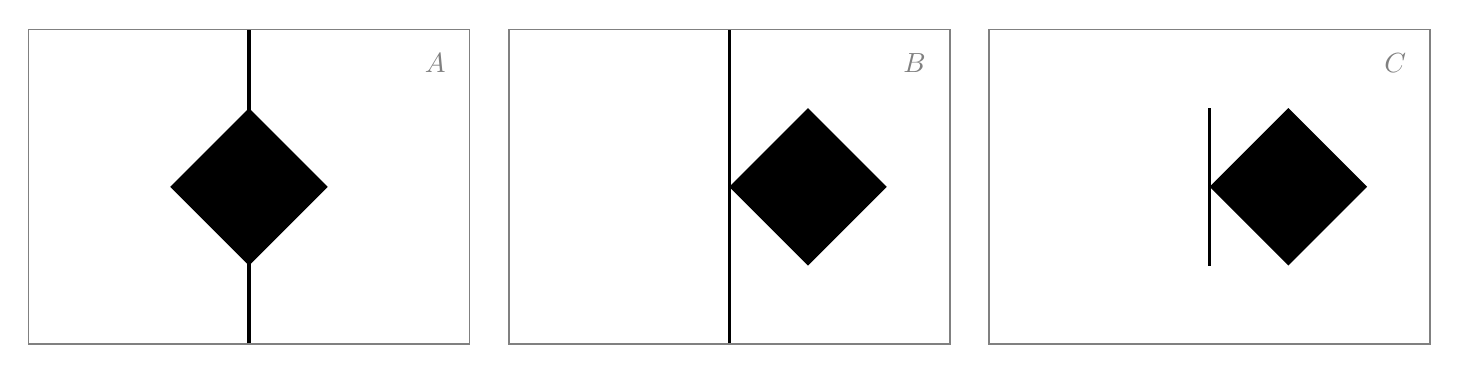
\begin{tikzpicture}
\draw[gray, line width=0.6pt] (-2.8,-2) rectangle (2.8,2) 
			node[anchor=north east, shift={(-5pt,-5pt)}]{$A$};	
\draw[black, line width=1.2pt, shorten <= 0.3pt, shorten >= 0.3pt] 
			(0,-2) -- (0,2);
\fill[black] (0,-1) -- (1,0) -- (0,1) -- (-1,0) -- cycle;
\begin{scope}[shift={(6.1,0)}]
\draw[gray, line width=0.6pt] (-2.8,-2) rectangle (2.8,2)
node[anchor=north east, shift={(-5pt,-5pt)}]{$B$};	
\draw[black, line width=1.2pt, shorten <= 0.3pt, shorten >= 0.3pt] 
(0,-2) -- (0,2);
\fill[black] (1,-1) -- (2,0) -- (1,1) -- (0,0) -- cycle;	
\end{scope}
\begin{scope}[shift={(12.2,0)}]
	\draw[gray, line width=0.6pt] (-2.8,-2) rectangle (2.8,2) 
	node[anchor=north east, shift={(-5pt,-5pt)}]{$C$};	
	\draw[black, line width=1.2pt] 
	(0,-1) -- (0,1);
	\fill[black] (1,-1) -- (2,0) -- (1,1) -- (0,0) -- cycle;	
\end{scope}
\end{tikzpicture}
\end{document}
